
\section{Appendix: Software Used}
\label{software_used}
Our application stack uses a variety of technologies and libraries in order to provide a cohesive environment for aggregating distributed power quality data. Our software is developed using Java, Scala, Javascript, and markup languages for display (CSS, HTML). We make heavy use of asynchronous communication by using the WebSocket protocol and use Twitter Bootstrap to provide a consistent and reactive user interface.

\subsection{Development Environment}
The OPQ Cloud software was developed on Debian GNU/Linux using version 7 of the OpenJDK. The software is shared under version 3 of the GPL license and all sources are shared on Github.

\subsection{Cloudbees}
Our OPQ Cloud application is hosted on Cloudbees which provides a platform as a service (PaaS) for building, running, and managing web applications. Cloudbees provides a continuous deployment environment which allows us to push changes to Github and Cloudbees will automatically build, run static analysis on the software, and deploy the software to the cloud. The Cloudbees web service can be found at \url{<http://www.cloudbees.com/>}.

\subsection{Play Framework}
The Play Framework is a modern open source model, view, controller (MVC) framework which allows developers to write web applications in either Java or Scala. The Play Framework provides facilities for asynchronous communication between clients using the built-in WebSocket standard. The Play Framework can be obtained at \url{<http://www.playframework.com/>}.

\subsection{Ebean ORM}
The Ebean object-relational mapping (ORM) is provided by the play framework and allows us to easily persist Plain Old Java Objects (POJOs) to the database of our choosing. Specifically, we are using MySQL as our database back end. Information about Ebean can be found at \url{<http://www.avaje.org/>}.

\subsection{Twitter Bootstrap}
Twitter Bootstrap is a library which consists of pre-rolled CSS, HTML, and Javascript templates for rapidly creating reactive and consistent user interfaces. Bootstrap allows us to create an interface that is consistent across multiple devices from desktops, to laptops, tablets, and mobile phones. Bootstrap can be downloaded at \url{<http://getbootstrap.com/>}.

\subsection{Fuel UX}
Fuel UX is a set of extensions built on top of Bootstrap that add extra functionality to Bootstrap driven websites. We're specifically using Fuel UX for the sign-up wizard in our OPQ cloud service. Fuel UX can be found at \url{<http://exacttarget.github.io/fuelux/>}.

\subsection{Leaflet}
Leaflet is an open source, mobile ready, Javascript library for creating interactive maps. We use Leaflet to display distributed PEs as well as for allowing users to select the location of their device as well as to allow users to select their neighborhood. We built an anonymous grid layer on top of Leaflet so that consumers can feel comfortable sharing their PQ data. Leaflet can be obtained at \url{<http://leafletjs.com/>}.

\subsection{OpenStreetMap}
OpenStreetMap provides a mapping service similar to Google Maps, but uses crowd sourced information to generate their maps and releases their map tiling images as open data. OPQ makes use of OpenStreetMap by using their tiling API within the Leaflet library. More information about OpenStreetMap can be found at \url{<http://www.openstreetmap.org/about>}.

\subsection{Java Websocket}
Java Websocket is an open source library which provides access to the Websocket Standard. This library is used by our OPQ Simulator to act as a client device. This library was not needed in the OPQ Cloud software as the Play framework handles all WebSocket communications for us. Java Websocket can be found at \url{<http://java-websocket.org/>}.

\subsection{JavaFX}
JavaFX is a graphical user interface (GUI) framework which provides tools from developing GUIs seamlessly across multiple different platforms and architectures. JavaFX makes integration with web technologies such as CSS and embedded HTML easy. We use JavaFX as the GUI back end to our OPQ simulator. JavaFX can be obtained at \url{<http://www.oracle.com/technetwork/java/javafx/overview/index.html>  }.

\subsection{Static Analysis}
We use a variety of static analysis tools to spot bugs in our source code. JUnit \url{<http://junit.org/>} is used as a unit testing framework for our software. FluentLenium \url{<http://fluentlenium.org/>} is used for writing acceptance tests for our software. We use FindBugs \url{<http://findbugs.sourceforge.net/>} to perform further static analysis and to enforce coding standards. Finally, we use Emma \url{<http://emma.sourceforge.net/>} to perform unit test coverage over our source code base.

\newpage

\section{Appendix: Screenshots}
% Wizard screenshots
\begin{figure}[htbp]
	\centering
	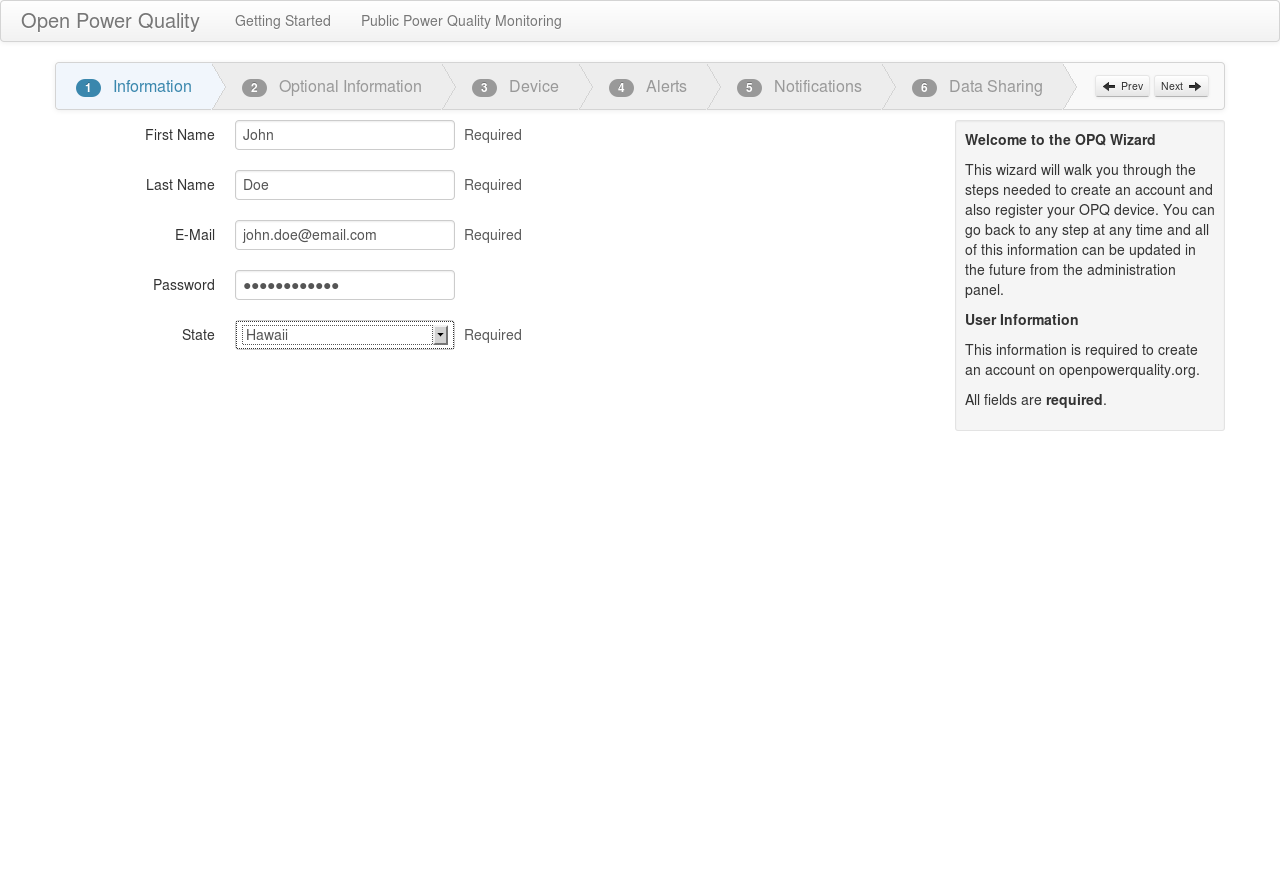
\includegraphics[width=\textwidth]{figures/wizard_1.eps}
	\caption{OPQ Wizard Screenshot.}
	\label{fig:wizard_1}
\end{figure}

\begin{figure}[htbp]
	\centering
	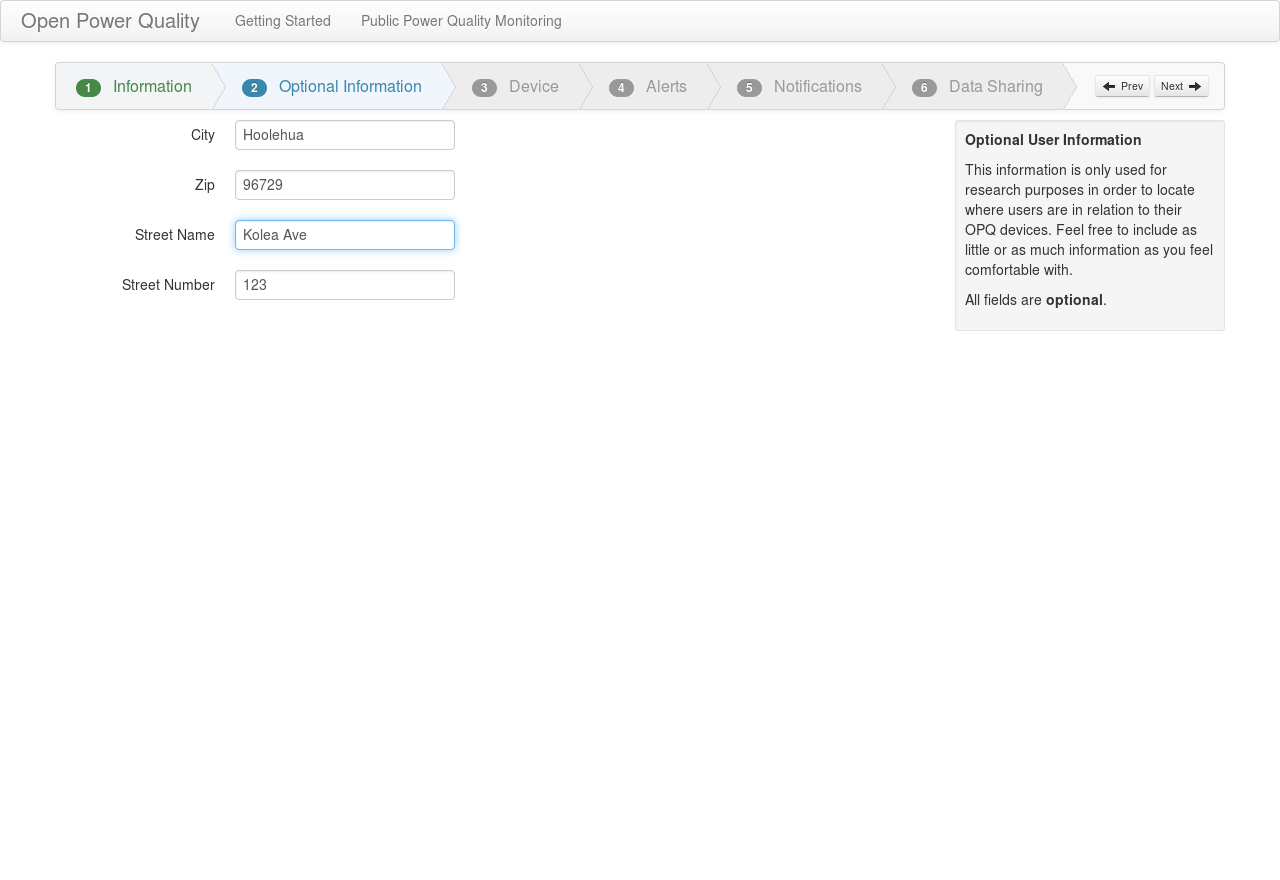
\includegraphics[width=\textwidth]{figures/wizard_2.eps}
	\caption{OPQ Wizard Screenshot.}
	\label{fig:wizard_2}
\end{figure}

\begin{figure}[htbp]
	\centering
	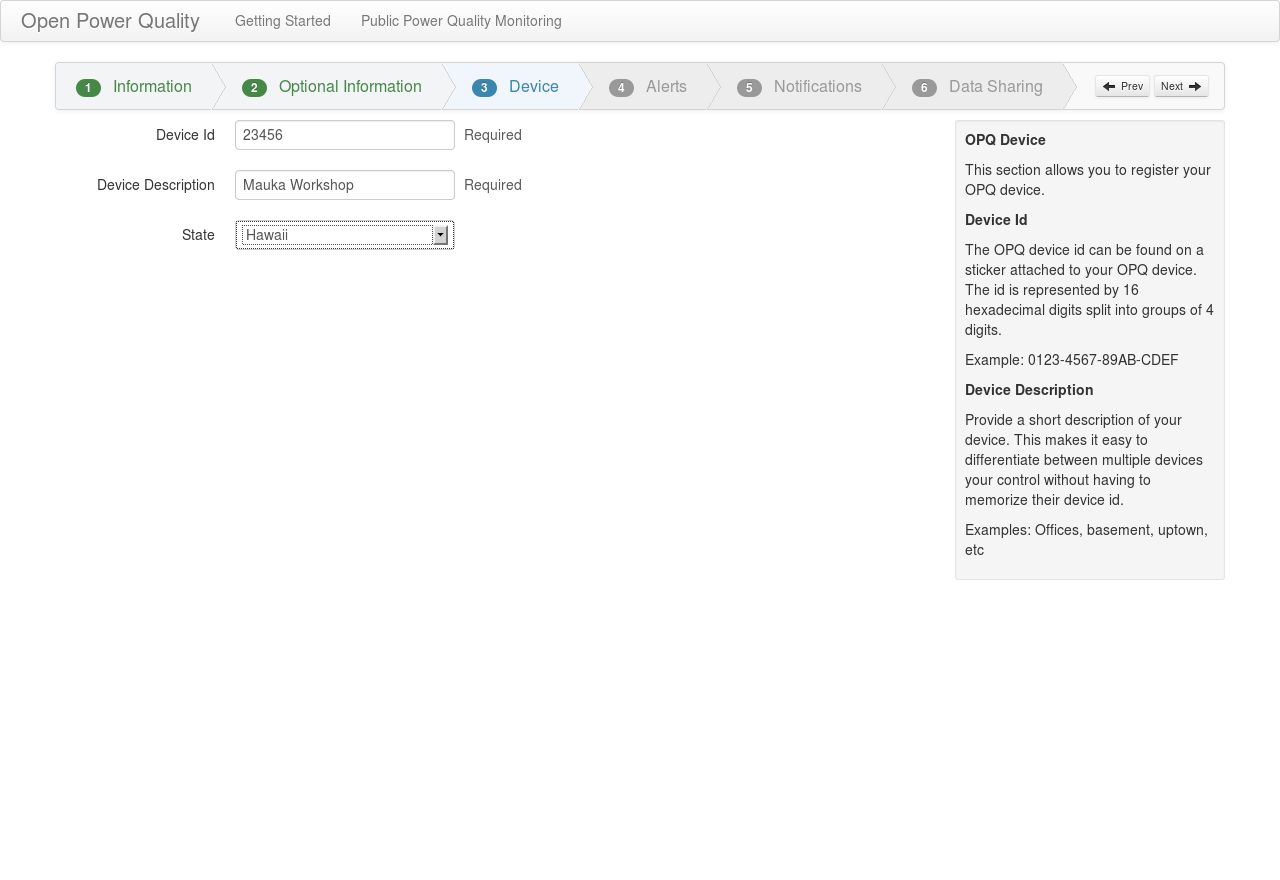
\includegraphics[width=\textwidth]{figures/wizard_3.eps}
	\caption{OPQ Wizard Screenshot.}
	\label{fig:wizard_3}
\end{figure}

\begin{figure}[htbp]
	\centering
	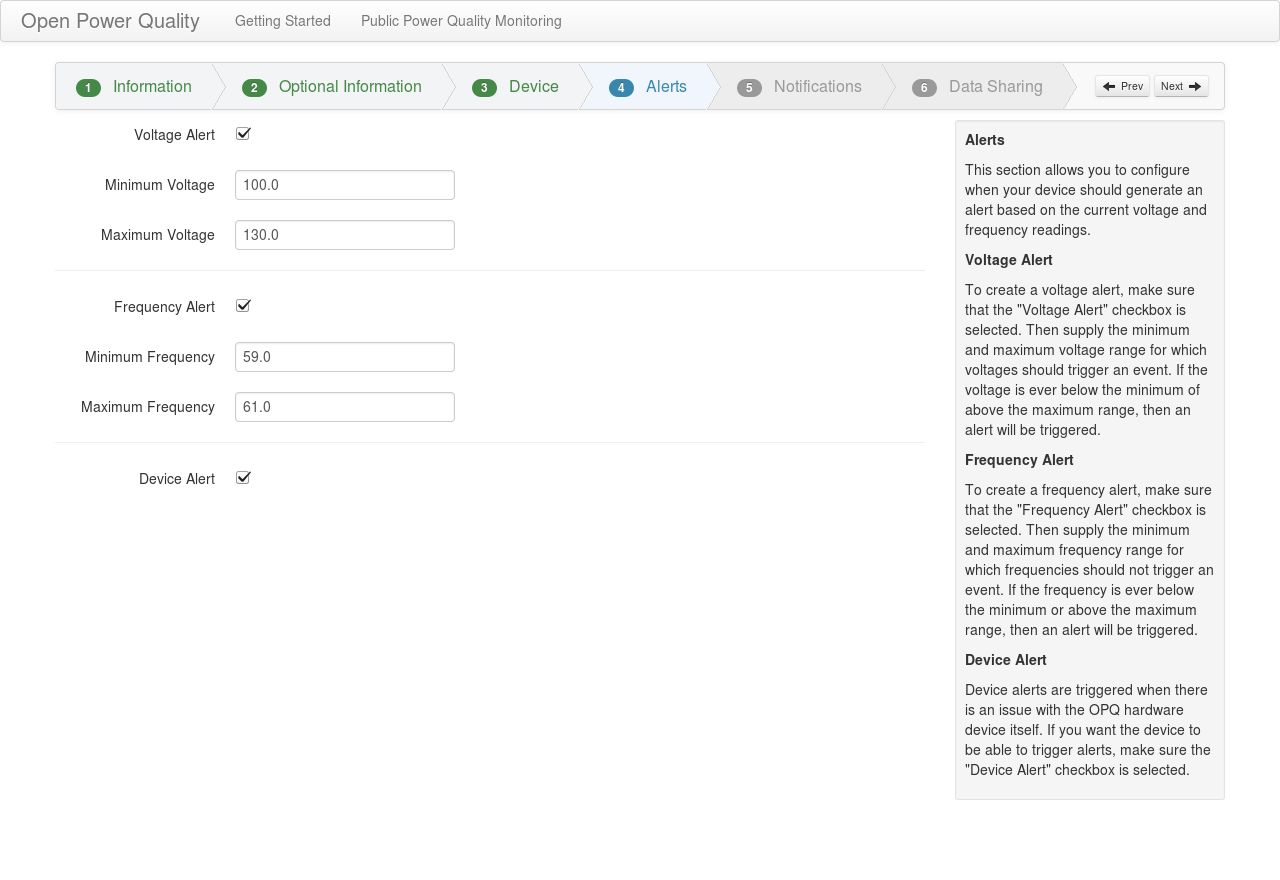
\includegraphics[width=\textwidth]{figures/wizard_4.eps}
	\caption{OPQ Wizard Screenshot.}
	\label{fig:wizard_4}
\end{figure}

\begin{figure}[htbp]
	\centering
	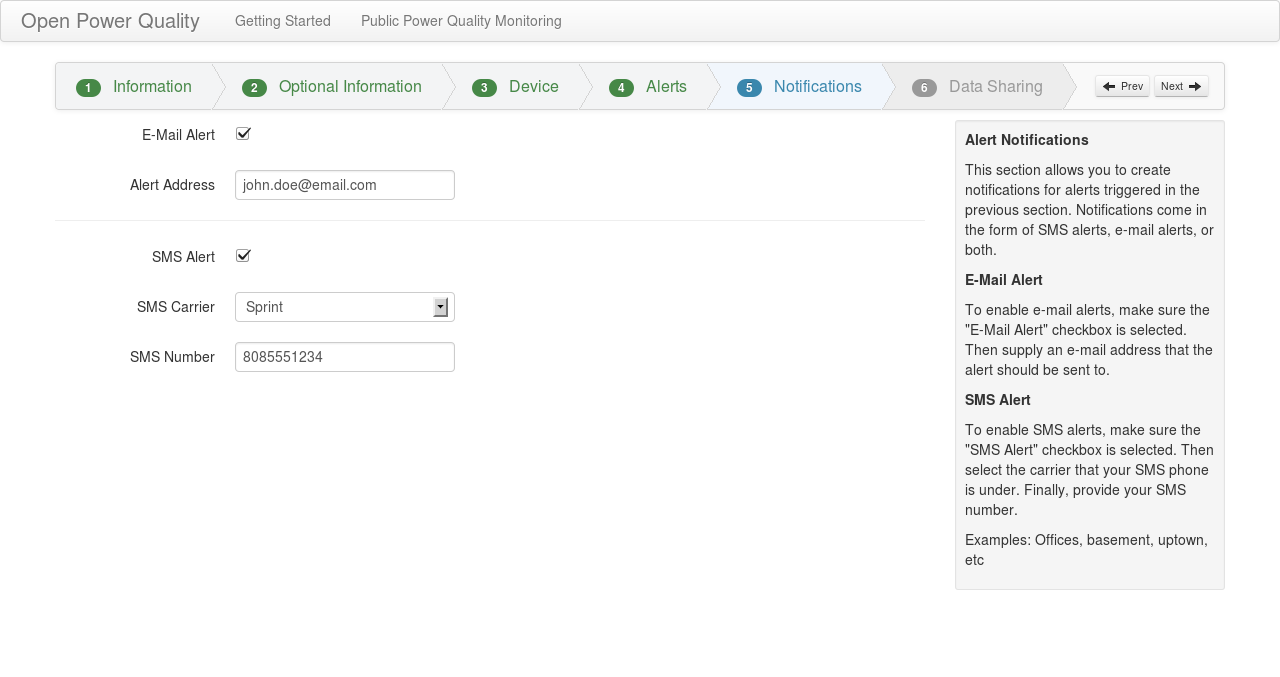
\includegraphics[width=\textwidth]{figures/wizard_5.eps}
	\caption{OPQ Wizard Screenshot.}
	\label{fig:wizard_5}
\end{figure}

\begin{figure}[htbp]
	\centering
	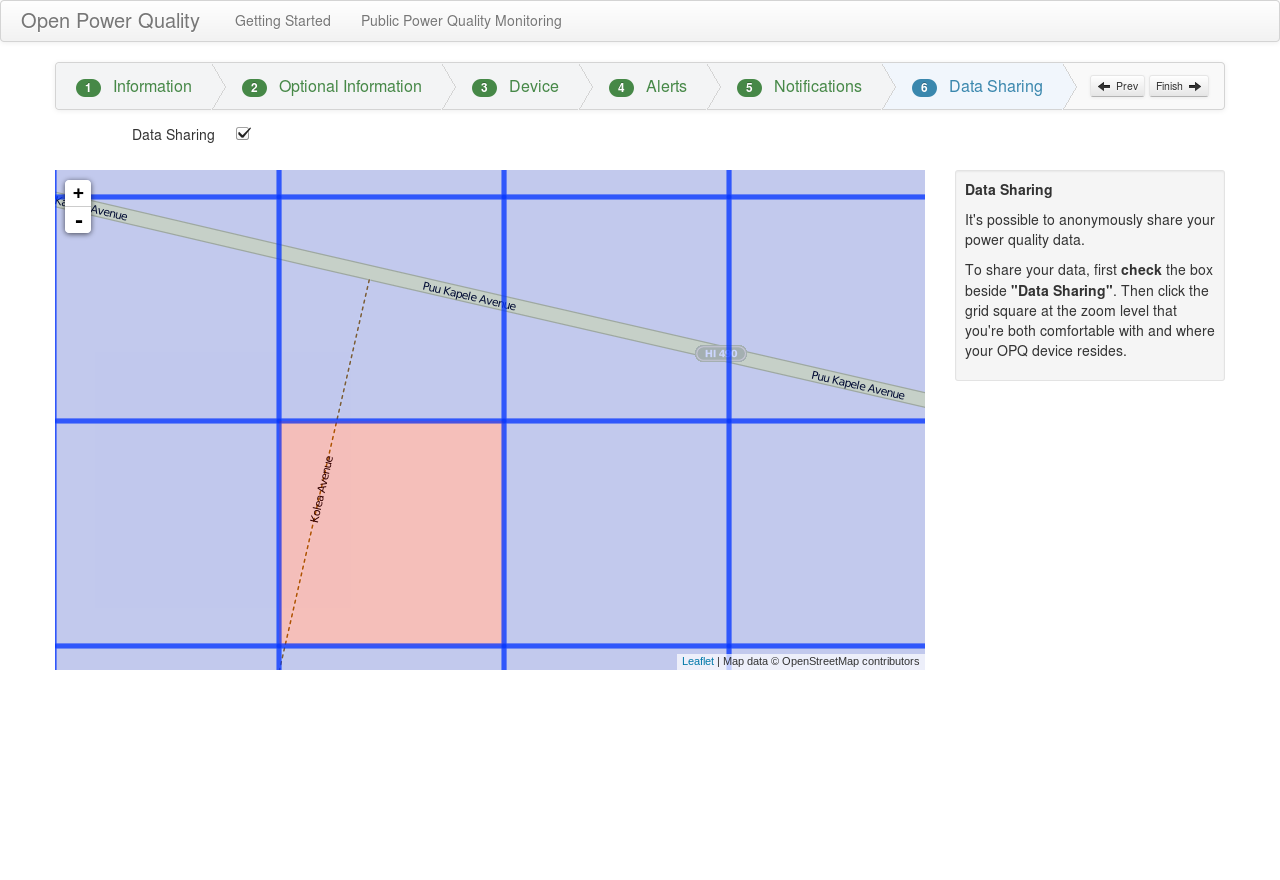
\includegraphics[width=\textwidth]{figures/wizard_6.eps}
	\caption{OPQ Wizard Screenshot.}
	\label{fig:wizard_6}
\end{figure}

% Private Measurements
\begin{figure}[htbp]
	\centering
	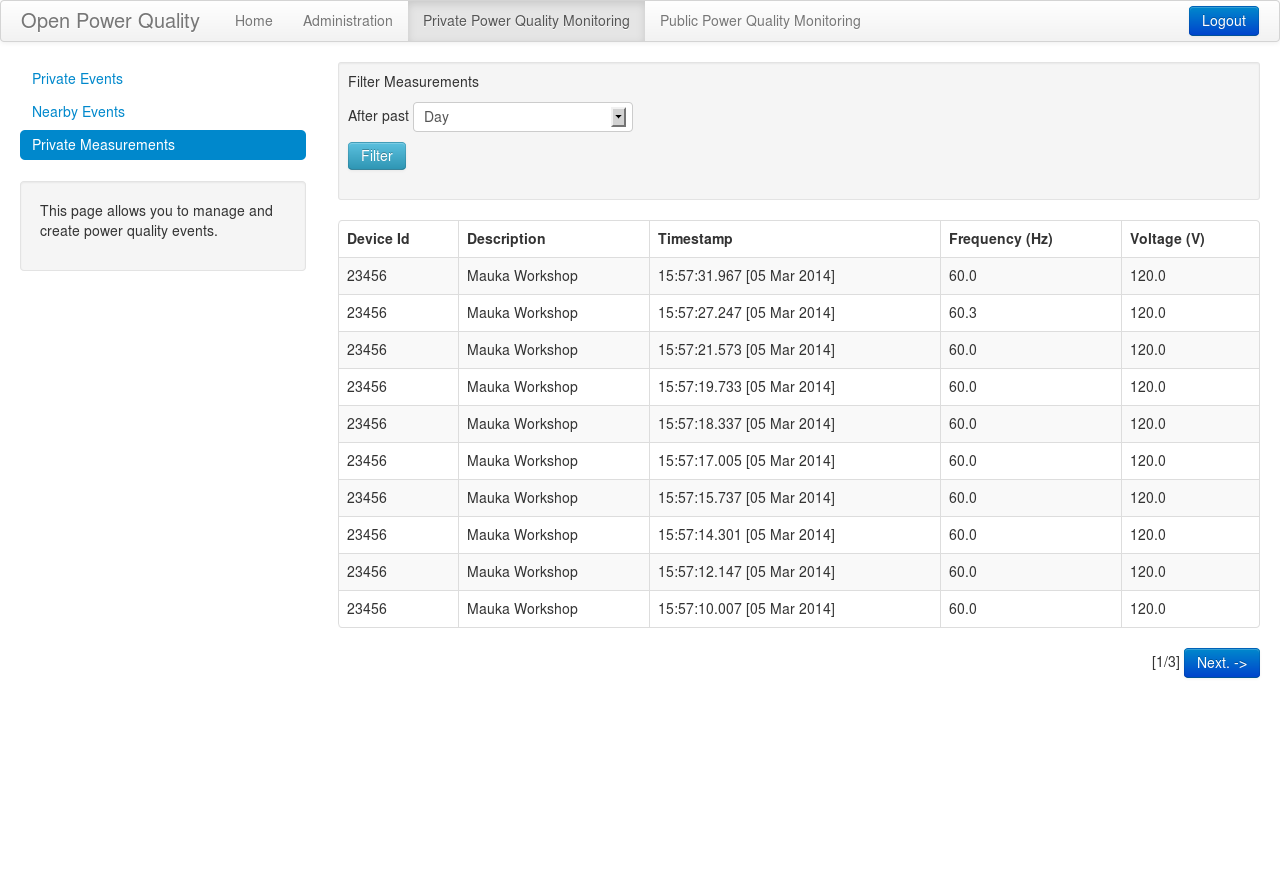
\includegraphics[width=\textwidth]{figures/private_measurements.eps}
	\caption{Private PQ Measurements.}
	\label{fig:private_measurements}
\end{figure}

% Private PQ Events
\begin{figure}[htbp]
	\centering
	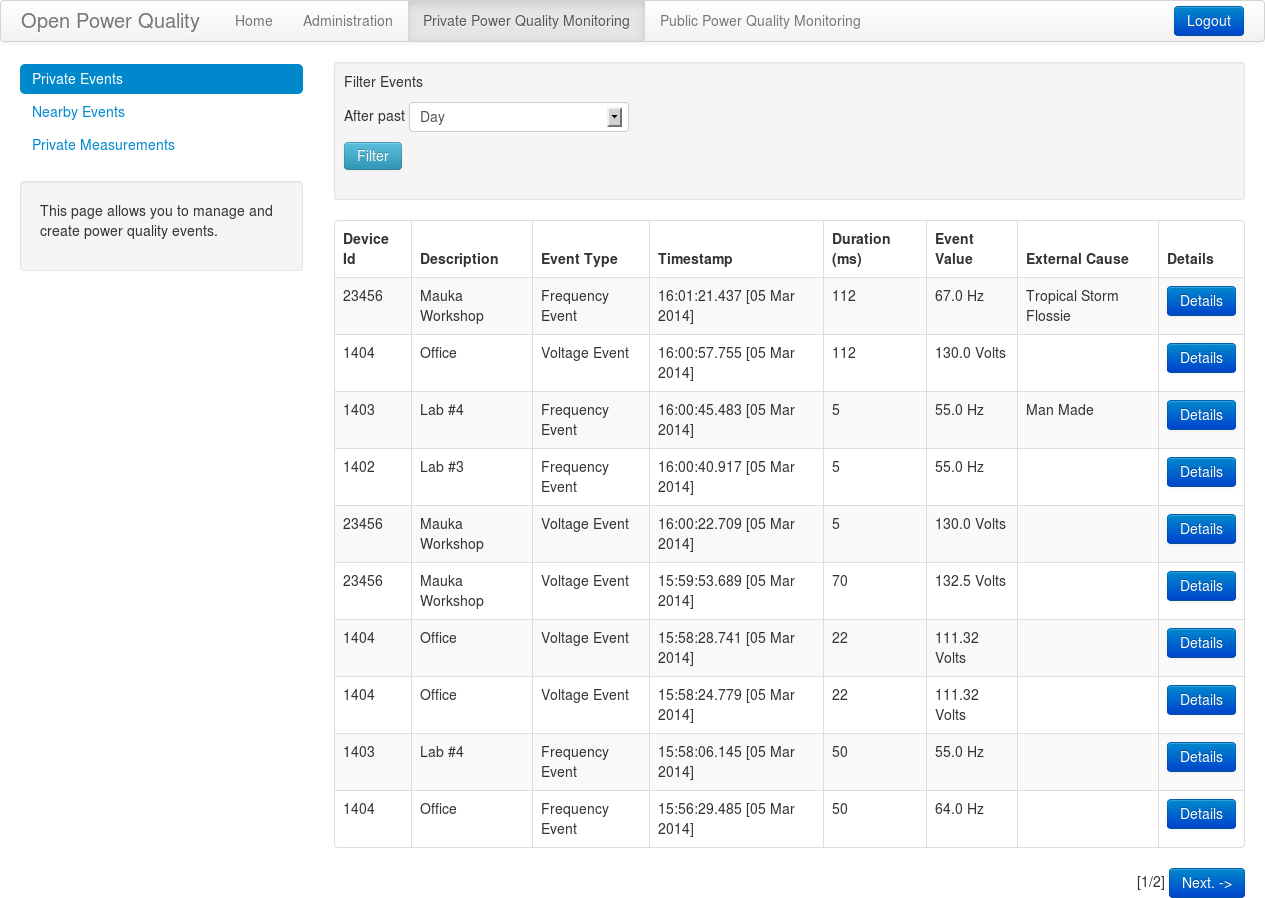
\includegraphics[width=\textwidth]{figures/private_events.eps}
	\caption{Private PQ Events.}
	\label{fig:private_events}
\end{figure}

% Nearby PQ event
\begin{figure}[htbp]
	\centering
	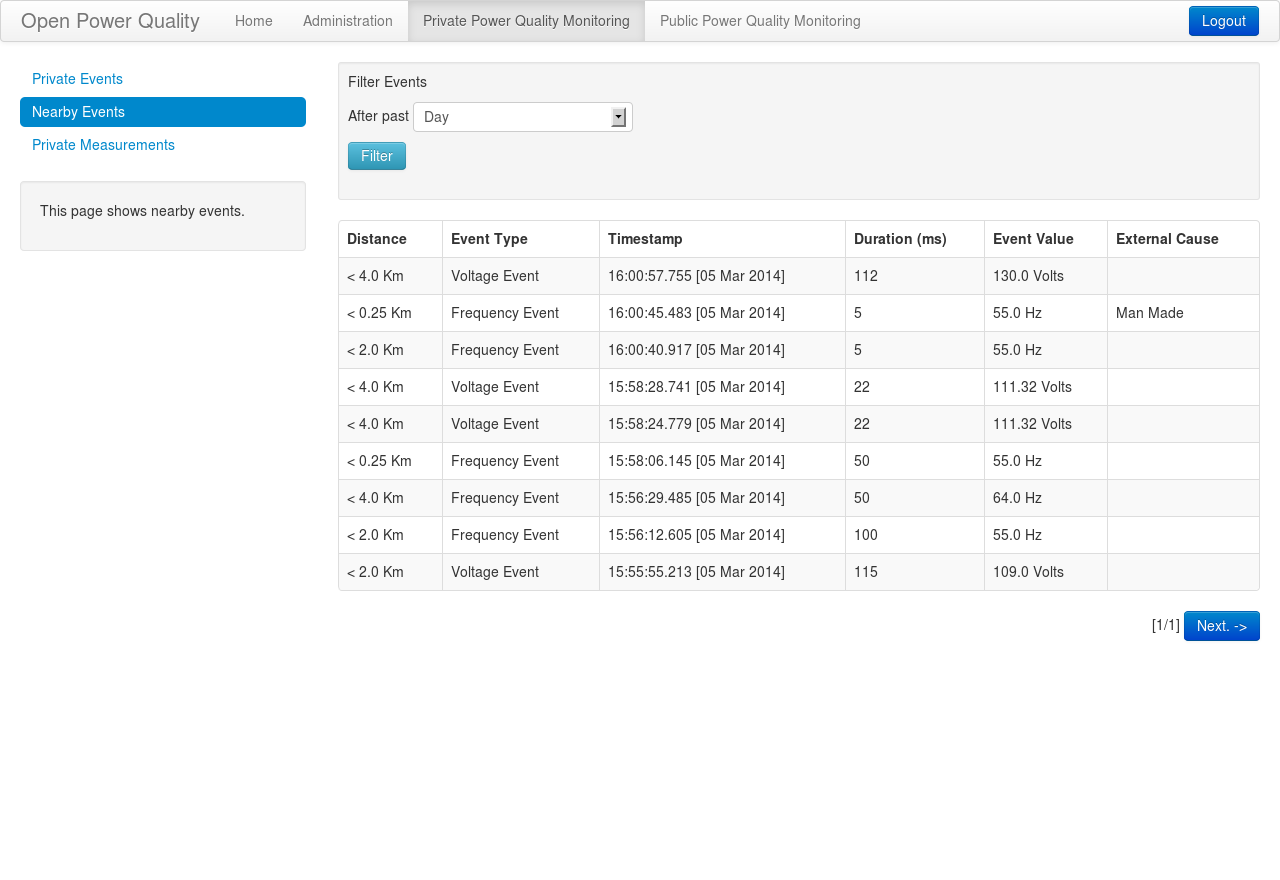
\includegraphics[width=\textwidth]{figures/private_nearby_events.eps}
	\caption{Nearby PQ Events.}
	\label{fig:nearby_events}
\end{figure}

% Alert admin
\begin{figure}[htbp]
	\centering
	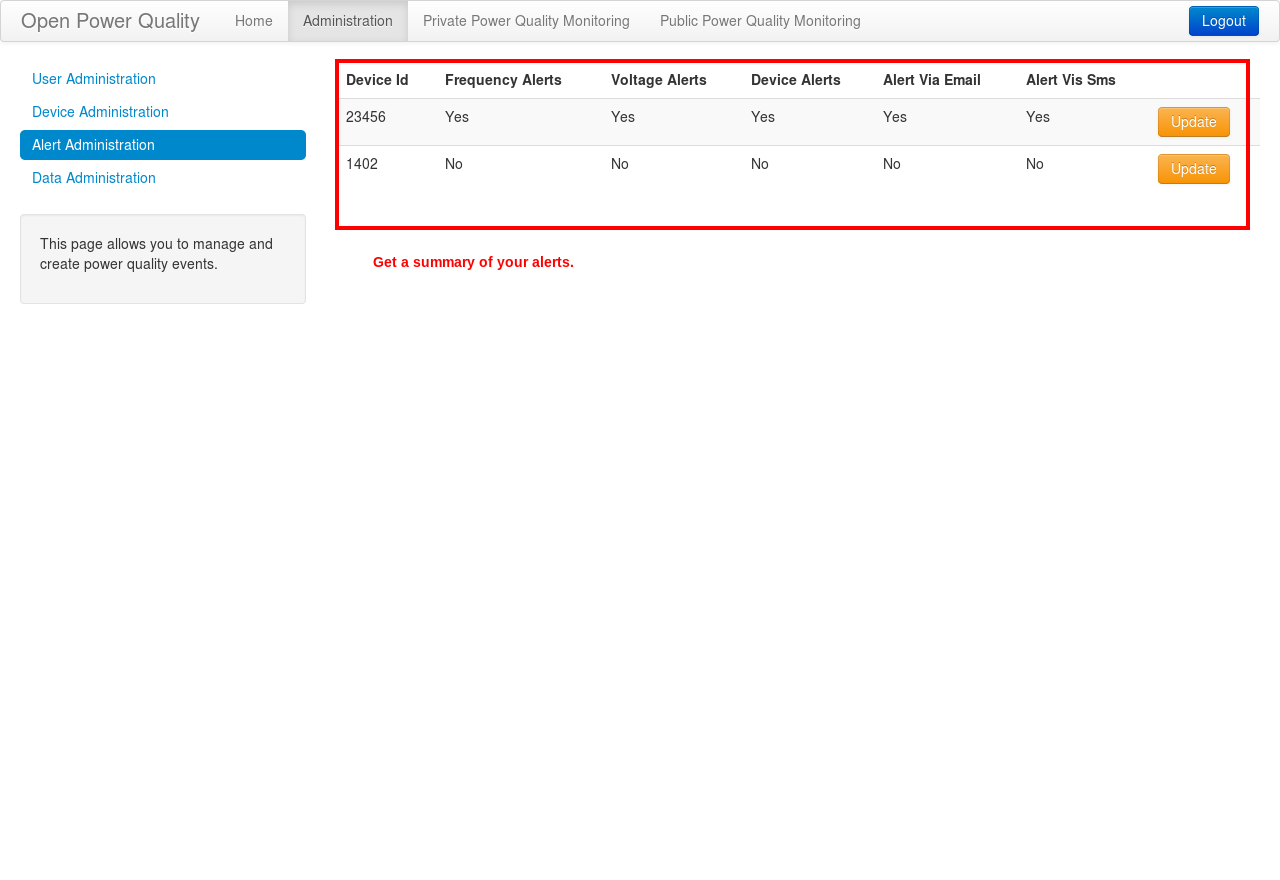
\includegraphics[width=\textwidth]{figures/alert_admin.eps}
	\caption{Alert Administration.}
	\label{fig:alert_admin}
\end{figure}

% Device admin
\begin{figure}[htbp]
	\centering
	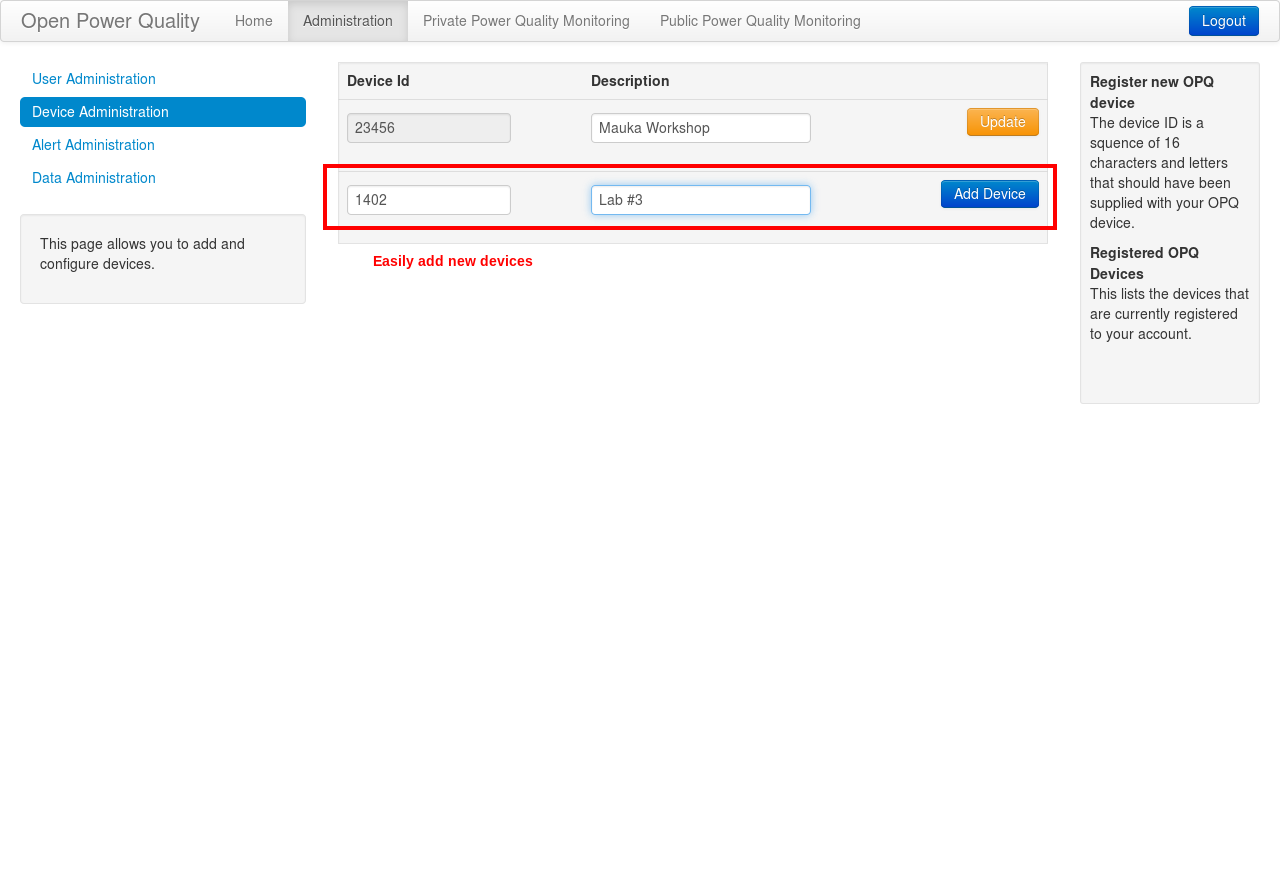
\includegraphics[width=\textwidth]{figures/device_admin.eps}
	\caption{Device Administration.}
	\label{fig:device_admin}
\end{figure}

% Simulator
\begin{figure}[htbp]
	\centering
	\includegraphics[width=\textwidth]{figures/sim_single_packet.eps}
	\caption{OPQ Simulator Single Packet}
	\label{fig:sim_single}
\end{figure}

\begin{figure}[htbp]
	\centering
	\includegraphics[width=\textwidth]{figures/sim_stress_test.eps}
	\caption{OPQ Simulator Stress Test Simulation}
	\label{fig:sim_multi}
\end{figure}
